\documentclass{beamer}
\usepackage[spanish]{babel}
\usepackage[latin1]{inputenc}
\usepackage{multicol} % indice en 2 columnas
\usepackage{centernot}
\usepackage{amsmath}% http://ctan.org/pkg/amsmath

\usepackage{color}


\usepackage{graphicx}
\graphicspath{ {im/} }


\newcommand{\notimplies}{%
  \mathrel{{\ooalign{\hidewidth$\not\phantom{=}$\hidewidth\cr$\implies$}}}}


\usetheme{Warsaw}
%\usecolortheme{crane}
\useoutertheme{shadow}
\useinnertheme{rectangles}

\setbeamertemplate{navigation symbols}{} % quitar simbolitos

\title[Tema 4 - Aplicaciones lineales]{Aplicaciones lineales}
\subtitle{Estudios de Ingenier\'ia}
\author[https://frogames.es]{
Juan Gabriel Gomila%$^{1}$  \and E. Eva$^{2}$ \and S. Serpiente$^{3}$
}
\institute[Frogames]{
 % $^{1-2}$
 Frogames
   \and
  \texttt{https://frogames.es}
}
\date{\today}

\AtBeginSection{
\begin{frame}
  \begin{multicols}{2}
  \tableofcontents[currentsection]   
\end{multicols}
\end{frame}
}

\AtBeginSubsection{
\begin{frame}
  \begin{multicols}{2}
  \tableofcontents[currentsection,currentsubsection]
\end{multicols}
\end{frame}
}



%empieza aqui


\begin{document} 

\frame{\titlepage}

\begin{frame}
  \frametitle{\'Indice}
  \tableofcontents
\end{frame}

\section{Definiciones b\'asicas}

\begin{frame}
  \frametitle{Definiciones b\'asicas}
  \begin{block}{Aplicaci\'on entre dos conjuntos}
Sean $A$ y $B$ dos conjuntos dados. Una \textbf{aplicaci\'on de $A$ en $B$} es una correspondencia que a cada elemento $x\in A$ le asocia un, y solo un, elemento $y\in B$ 
\end{block}

\begin{figure}[h]
  \label{fig:esquema}
  \caption{Ejemplos de correspondencias que no son aplicaciones}
\centering
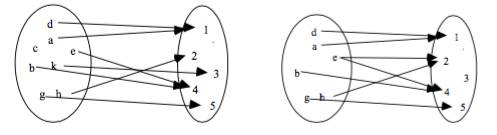
\includegraphics[width=\textwidth]{no_aplicacio}
\end{figure}
\end{frame}




\begin{frame}
  \frametitle{Definiciones b\'asicas}
  \begin{block}{Aplicaci\'on exhaustiva}
Sea $f:A\longrightarrow B$ una aplicaci\'on. D\'icese que $f$ es \textbf{exhaustiva} si y solo si $f(A) = B$. Es decir, si todos los elementos de $B$ tienen una anti-imagen o antecedente.
\[\forall\ b\in B \exists \ a\in A\ : \ f(a) = b\]
\end{block}
\end{frame}

\begin{frame}
  \frametitle{Definiciones b\'asicas}
\begin{figure}[h]
  \label{fig:esquema}
  \caption{La aplicaci\'on de la izquierda es exhaustiva. La de la derecha no lo es (el n\'umero 3 no tiene ninguna anti-imagen)}
\centering
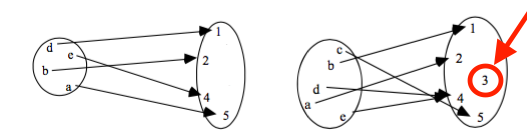
\includegraphics[width=\textwidth]{exhaustiva}
\end{figure}
\end{frame}



\begin{frame}
  \frametitle{Definiciones b\'asicas}
  \begin{block}{Aplicaci\'on exhaustiva}
Sea $f:A\longrightarrow B$ una aplicaci\'on. Se dice que $f$ es \textbf{inyectiva} si distintos elementos de $A$ tienen distinta imagen.
\[x,y\in A, \ x\neq y \Rightarrow  f(x) \neq f(y)\]
Esto es equivalente a decir que si dos elementos tienen la misma imagen para $f$ entonces son el mismo elemento:
\[f(x) = f(y) \Rightarrow x = y\]
\end{block}
\end{frame}



\begin{frame}
  \frametitle{Definiciones b\'asicas}
De la definici\'on anterior se deduce que cada elemento de $B$ tendr\'a como m\'aximo una anti-imagen. En otras palabras, la anti-imagen de un elemento de $B$ es o bien un elemento de $A$ o bien el conjunto vac\'io.
\end{frame}

\begin{frame}
  \frametitle{Definiciones b\'asicas}
\begin{figure}[h]
  \label{fig:esquema}
  \caption{La aplicaci\'on de la izquierda es inyectiva. La de la derecha no lo es (el n\'umero 4 tiene dos anti-im\'agenes para $f$).}
\centering
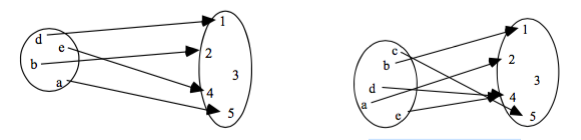
\includegraphics[width=\textwidth]{injectiva}
\end{figure}
\end{frame}



\begin{frame}
  \frametitle{Definiciones b\'asicas}
  \begin{block}{Aplicaci\'on biyectiva}
Sea $f:A\longrightarrow B$ una aplicaci\'on. D\'icese que $f$ es \textbf{biyectiva} si es inyectiva y exhaustiva a la vez. El concepto equivale a decir que:
\[\forall\ b\in B\ \exists ! a\in A\ : \ f(a) = b\]
\end{block}
\end{frame}

\begin{frame}
  \frametitle{Definiciones b\'asicas}
\begin{figure}[h]
  \label{fig:esquema}
  \caption{Todo elemento de $B$ tiene una, y solo una, \'unica anti-imagen para $f$}
\centering
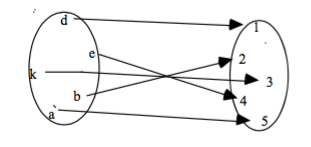
\includegraphics[scale=0.7]{bijectiva}
\end{figure}
\end{frame}


\section{Aplicaciones lineales}
\subsection{La aplicaci\'on identidad}
\begin{frame}
  \frametitle{La aplicaci\'on identidad}

Consid\'erese un espacio vectorial $E$ y la aplicaci\'on identidad que transforma cada vector de $E$ en \'el mismo:   
  
  \[
  \begin{array}{@{}r@{\;}c@{\;}c@{\;}l@{}}
    I: & E & \rightarrow & E,   \\
       & x & \mapsto     & x.
  \end{array}
\]
En primer lugar se estudiar\'a si existe alguna relaci\'on entre la imagen de una suma de vectores $I(x+y)$ y las im\'agenes de cada uno de los sumandos $I(x),I(y)$. 

\end{frame}

\begin{frame}
  \frametitle{La aplicaci\'on identidad - Lineal para la suma}

Por definici\'on de la aplicaci\'on identidad:
  \[
I(x+y) = x+y
\]
Por otro lado:
\[\left.\begin{array}{ccc}I(x) & = & x \\I(y) & =  & y\end{array}\right\} \Rightarrow I(x)+I(y) = x+y\]
Y por tanto se puede escribir que:
\[I(x+y) = x+y = I(x)+I(y)\]
 \begin{block}{Aplicaci\'on lineal para la suma}
La imagen de la suma es la suma de im\'agenes.
\end{block}

\end{frame}


\begin{frame}
  \frametitle{La aplicaci\'on identidad - Lineal para el producto por escalar}

En segundo lugar se estudiar\'a si existe alguna relaci\'on entre la imagen de un escalar por un vector $I(\lambda x)$ y la imagen del vector $I(x)$. 

Por definici\'on de aplicaci\'on identidad:
  \[
I(\lambda x) = \lambda x
\]
Por tanto podemos escribir que:
\[I(\lambda x) = \lambda x= \lambda I(x)\]
 \begin{block}{Aplicaci\'on lineal para el producto por escalar}
La imagen del producto de un escalar por un vector es el escalar por la imagen del vector.
\end{block}
\end{frame}

\subsection{La aplicaci\'on constante}
\begin{frame}
  \frametitle{La aplicaci\'on constante}

Se ver\'a ahora la aplicaci\'on definida en $\mathbb R$ que transforma cada n\'umero real en el n\'umero $2$  
  \[
  \begin{array}{@{}r@{\;}c@{\;}c@{\;}l@{}}
    f: & \mathbb R & \rightarrow & \mathbb R,   \\
       & x & \mapsto     & 2.
  \end{array}
\]
Como antes, se va a estudiar la relaci\'on entre la imagen de una suma de vectores $f(x+y)$ y las im\'agenes de cada uno de los sumandos $f(x),f(y)$. 

\end{frame}


\begin{frame}
  \frametitle{La aplicaci\'on constante - Lineal para la suma}

Por definici\'on de la aplicaci\'on constante:  
  \[
f(x+y) = 2
\]
Por otro lado:
\[\left.\begin{array}{ccc}f(x) & = & 2 \\f(y) & =  & 2\end{array}\right\} \Rightarrow f(x)+f(y) = 2+2=4\]
Y por tanto se puede escribir que:
\[f(x+y) = 2  \neq 4 = f(x)+f(y)\]
 \begin{block}{Aplicaci\'on no lineal para la suma}
La imagen de la suma \textbf{NO} es la suma de im\'agenes.
\end{block}

\end{frame}

\begin{frame}
  \frametitle{La aplicaci\'on constante - Lineal para el producto por escalar}

En segundo lugar se estudiar\'a si existe alguna relaci\'on entre la imagen de un escalar por un vector $f(\lambda x)$ y la imagen del vector $f(x)$. 

Por definici\'on de la aplicaci\'on constante:
  \[
f(\lambda x) = 2
\]
Por tanto podemos escribir que:
\[f(\lambda x) = 2 \neq 2 \lambda = \lambda f(x)\]
 \begin{block}{Aplicaci\'on no lineal para el producto por escalar}
La imagen del producto de un escalar por un vector \textbf{NO} es el escalar por la imagen del vector.
\end{block}
\end{frame}


\subsection{Definici\'on de aplicaci\'on lineal}


\begin{frame}
  \frametitle{Aplicaci\'on lineal}
La aplicaci\'on identidad del primer ejemplo es una \textbf{aplicaci\'on lineal}.

La apliaci\'on constante del segundo ejemplo NO es una \textbf{aplicaci\'on lineal}.
\end{frame}



\begin{frame}
  \frametitle{Aplicaci\'on lineal}
 \begin{block}{Aplicaci\'on  lineal}
Sea $E$ y $F$ dos espacios vectoriales sobre $\mathbb K$. T\'engase una aplicaci\'on $f$ dada por:
  \[
  \begin{array}{@{}r@{\;}c@{\;}c@{\;}l@{}}
    f: & E & \rightarrow & F,   \\
       & x & \mapsto     & f(x).
  \end{array}
\]
D\'icese que $f$ es una aplicaci\'on lineal si se verifica que:
\begin{enumerate}
\item $\forall\ \vec x,\vec y \in E, \ \ f(\vec x + \vec y) = f(\vec x) + f(\vec y)$
\item $\forall\ \lambda\in\mathbb K,\ \ \forall \vec x \in E, \ \ f(\lambda \vec x) = \lambda f(\vec x)$
\end{enumerate}
\end{block}
\end{frame}

\begin{frame}
  \frametitle{Aplicaci\'on lineal}
Las dos condiciones anteriores son equivalentes a una tercera:
 \begin{block}{Aplicaci\'on  lineal(II)} 
\[\forall\ \lambda,\mu \in\mathbb K, \vec x,\vec y \in E, \ \ f(\vec \lambda x + \mu \vec y) = \lambda f(\vec x) + \mu f(\vec y)\]
\end{block}

Normalmente comprobar las dos condiciones por separado suele ser m\'as sencillo a la hora de realizar operaciones. Comprobar una sola puede ahorrar tiempo pero habr\'a que tener cuidado pues a partir de ahora se tendr\'an m\'as variables que en el primer caso.
\end{frame}



\begin{frame}
  \frametitle{Aplicaci\'on lineal}
 \begin{block}{Ejercicios} 
Estudiar si la siguiente aplicaci\'on es o no lineal:
  \[
  \begin{array}{@{}r@{\;}c@{\;}c@{\;}l@{}}
    f: & \mathbb K^2 & \rightarrow & \mathbb K,   \\
       & (x,y) & \mapsto     & x.
  \end{array}
\]
Esta aplicaci\'on recibe el nombre de \textbf{primera proyecci\'on}.
\end{block}

\end{frame}


\begin{frame}
  \frametitle{Aplicaci\'on lineal}
  \begin{enumerate}
  \item Lineal para la suma
\[f((x_1, y_1)+(x_2,y_2)) = f(x_1+x_2, y_1+y_2) = x_1+x_2\]
\[\left.\begin{array}{ccc}f(x_1,y_1) & = & x_1 \\f(x_2,y_2) & =  & x_2\end{array}\right\} \Rightarrow f(x_1,y_1)+f(x_2,y_2) = x_1+x_2\]
Y por lo tanto:
\[f((x_1, y_1)+(x_2,y_2)) = x_1+x_2 = f(x_1,y_1)+f(x_2,y_2)\]

\item Lineal para el producto por escalar
\[f(\lambda(x,y)) = f(\lambda x, \lambda y) = \lambda x = \lambda f(x,y)\]
\end{enumerate}
\end{frame}

\subsection{Propiedades}
\begin{frame}
  \frametitle{Preguntas}
?`Cu\'ando se dice que una aplicaci\'on es lineal? 
 \[
  \begin{array}{@{}r@{\;}c@{\;}c@{\;}l@{}}
    f: & E & \rightarrow & F,   \\
       & x & \mapsto     & f(x).
  \end{array}
\]
Se va a intentar responder a preguntas del estilo:
  \begin{enumerate}
  \item ?`Cu\'al ser\'a la imagen del elemento neutro de $E$? 
  \item ?`Existe una relaci\'on entre la imagen de un vector $f(\vec x)$ y la de su opuesto $f(-\vec x)$?  
\end{enumerate}
Estas preguntas surgen de forma natural debido a las particularidades de $E$ por ser un espacio vectorial (contiene el neutro, los opuestos...). 
\end{frame}

\begin{frame}
  \frametitle{Preguntas}
Ve\'amoslo con el siguiente ejemplo de la primera proyecci\'on anterior, que asocia a cada vector su primera coordenada:
  \[
  \begin{array}{@{}r@{\;}c@{\;}c@{\;}l@{}}
    f: & \mathbb K^2 & \rightarrow & \mathbb K,   \\
       & (x,y) & \mapsto     & x.
  \end{array}
\]
  \begin{enumerate}
  \item La aplicac\'on env\'ia el vector nulo $\vec 0_E = (0,0)$ a su primera coordenada que es el n\'umero cero: $f(0,0) = 0$. Es decir, la imagen del vector nulo de $\mathbb K^2$ es el vector nulo de $\mathbb K$. ?`Ser\'a siempre as\'i?
  \item Como $f(-x,-y) = -x$ y $f(x,y) = x$, entonces $f(-x,-y) = -x, = -f(x,y)$. Es decir, la imagen del vector opuesto de un vector $\vec\in E$ Es el opuesto de la imagen de $\vec v$ por $f$. ?`Ser\'a siempre as\'i? 
\end{enumerate}
\end{frame}


\begin{frame}
  \frametitle{La imagen del vector nulo}
 \begin{block}{Propiedad} 
Dada una aplicaci\'on lineal
  \[
  \begin{array}{@{}r@{\;}c@{\;}c@{\;}l@{}}
    f: & E & \rightarrow & F,   \\
       & x & \mapsto     & f(x).
  \end{array}
\]
La imagen del vector nulo $\vec 0_E$ de $E$ es el vector nulo $\vec 0_F$ de $F$
\[f(\vec 0_E) = \vec 0_F\]
\end{block} 
 \end{frame}
 
 
\begin{frame}
  \frametitle{La imagen del vector nulo}
 \begin{block}{Demostraci\'on} 

\begin{enumerate}
\item El vector nulo $\vec 0_E$ es el neutro de la suma de $E$, por tanto:
\[\forall \vec x \in E \Rightarrow \vec x + \vec 0_E = \vec x\]
\item Como $\vec x + \vec 0_E = \vec x$, entonces: $f(\vec x + \vec 0_E) = f(\vec x)$.
\item Como $f$ es lineal: $f(\vec x + \vec 0_E) = f(\vec x) + f(\vec 0_E)$.
\item Entonces de 2 y 3, se obtiene: $f(\vec x)+ f(\vec 0_E) = f(\vec x)$
Donde, en efecto $f(\vec 0_E)$ es el elemento neutro de la suma de $F$: 
\[f(\vec 0_E) = \vec 0_F\]
\end{enumerate}
\end{block} 
 \end{frame}
 
 \begin{frame}
  \frametitle{La imagen del vector opuesto}
 \begin{block}{Propiedad} 
Dada una aplicaci\'on lineal:
  \[
  \begin{array}{@{}r@{\;}c@{\;}c@{\;}l@{}}
    f: & E & \rightarrow & F,   \\
       & x & \mapsto     & f(x).
  \end{array}
\]
La imagen del vector opuesto es el opuesto de la imagen del vector original:
\[f(-\vec x) = -f(\vec x)\]
\end{block} 
 \end{frame}
 
 
\begin{frame}
  \frametitle{La imagen del vector opuesto}
 \begin{block}{Demostraci\'on} 

\begin{enumerate}
\item La suma de un vector y su opuesto es el elemento neutro.
\[\forall \vec x \in E \Rightarrow \vec x + (-\vec x) = \vec 0_E\]
\item Como $\vec x + (-\vec x) = \vec 0_E$, entonces: $f(\vec x + (-\vec x)) = f(\vec 0_E)$.
\item Como $f$ es lineal: $f(\vec x + (-\vec x)) = f(\vec x) + f(-\vec x)$.
\item Entonces de 2 y 3, se obtiene: $f(\vec x)+ f(-\vec x) = f(\vec 0_E)$
\item Pero de la propiedad anterior se sabe que $f(\vec 0_E) = \vec 0_F$, y por tanto $f(\vec x) + f(-\vec x) = \vec 0_F$
Donde, por propiedad del elemento neutro $f(-\vec x)$ ha de ser el opuesto de $f(\vec x)$: 
\[f(-\vec x) = -f(\vec x)\]
\end{enumerate}
\end{block} 
 \end{frame}
 

\section{N\'ucleo, imagen y rango de una aplicaci\'on lineal}

\subsection{N\'ucleo}

\begin{frame}
  \frametitle{N\'ucleo de una aplicaci\'on lineal}
 \begin{block}{Definici\'on} 
Sea la aplicaci\'on lineal \[
  \begin{array}{@{}r@{\;}c@{\;}c@{\;}l@{}}
    f: & E & \rightarrow & F,   \\
       & x & \mapsto     & f(x).
  \end{array}
\] 
Se denomina \textbf{n\'ucleo de $f$} y se denota como $Ker(f)$ o $Nuc(f)$ el conjunto de elementos de $E$ tales que su imagen coincide con el cero de $F$:
\[Ker(f) = \{\vec x\in E\ : \ f(\vec x) = \vec 0_F\}\]
\end{block} 
 \end{frame}



\begin{frame}
  \frametitle{N\'ucleo de una aplicaci\'on lineal}
 \begin{block}{Teorema} 
Sea la aplicaci\'on lineal \[
  \begin{array}{@{}r@{\;}c@{\;}c@{\;}l@{}}
    f: & E & \rightarrow & F,   \\
       & x & \mapsto     & f(x).
  \end{array}
\] 
Entonces el $Ker(f)$ es un subespacio vectorial de $E$.
\end{block} 
 \end{frame}
 
 
\begin{frame}
  \frametitle{N\'ucleo de una aplicaci\'on lineal}
 \begin{block}{Ejercicios} 
Sea la aplicaci\'on lineal \[
  \begin{array}{@{}r@{\;}c@{\;}c@{\;}l@{}}
    f: & \mathbb R^3 & \rightarrow & \mathbb R^2,   \\
       & (x,y,z) & \mapsto     & (x+y-2z, x-y+z).
  \end{array}
\] 
H\'allese el $Ker(f)$ y una nueva base suya.
\end{block} 
 \end{frame}
 
 \begin{frame}
  \frametitle{N\'ucleo de una aplicaci\'on lineal}
 \begin{block}{Soluci\'on} 
Un elemente del n\'ucleo de $f$ cumple la ecuaci\'on:
 \[ f(x,y,z) = (x+y-2z, x-y+z)=(0,0)\] 
Si se resuelve el sistema pertinente se obtiene que:
\[x=x, y=3x, z=2x\]
Donde:
\[Ker(f) = \{(x,y,z)\in\mathbb R^3: y=3x, z=2x\} = \langle (1,3,2) \rangle\]
\end{block} 
 \end{frame}

\begin{frame}
  \frametitle{N\'ucleo de una aplicaci\'on lineal}
 \begin{block}{Teorema} 
Una aplicaci\'on lineal $f:E\rightarrow F$ es inyectiva si y solo si el n\'ucleo de $f$ se reduce al neutro de $E$.
\[f\ inyectiva \Longleftrightarrow Ker(f) = \{\vec 0_E\} \]
\end{block} 
 \end{frame}

\begin{frame}
\frametitle{N\'ucleo de una aplicaci\'on lineal}
\begin{block}{Teorema} 
Sea: 
\[\vec x_1, \vec x_2, \cdots \vec x_n\]
 Un conjunto de vectores linealmente independientes del espacio vectorial $E$ y $f:E\rightarrow F$ es una aplicaci\'on lineal inyectiva entonces: 
 \[f(\vec x_1), f(\vec x_2), \cdots, f(\vec x_n)\]
  Son vectores linealmente independientes pertenecientes a $F$. 
\end{block} 
 \end{frame}

\subsection{Imagen}


\begin{frame}
  \frametitle{Imagen de una aplicaci\'on lineal}
 \begin{block}{Definici\'on} 
Sea la aplicaci\'on lineal\[
  \begin{array}{@{}r@{\;}c@{\;}c@{\;}l@{}}
    f: & E & \rightarrow & F,   \\
       & x & \mapsto     & f(x).
  \end{array}
\] 
Se denomina \textbf{imagen de $f$} y se denota por $Im(f)$ al conjunto de elementos de $F$ que tienen una anti-imagen para $f$:
\[Im(f) = \{\vec y\in F\ : \exists \vec x \in E\ \ tq \ f(\vec x) = \vec y\}\]
\end{block} 
 \end{frame}

\begin{frame}
  \frametitle{Imagen de una aplicaci\'on lineal}
 \begin{block}{Teorema} 
T\'engase la aplicaci\'on lineal:\[
  \begin{array}{@{}r@{\;}c@{\;}c@{\;}l@{}}
    f: & E & \rightarrow & F,   \\
       & x & \mapsto     & f(x).
  \end{array}
\] 
Entonces el $Im(f)$ es un subespacio vectorial de $E$.
\end{block} 
 \end{frame}
 



\begin{frame}
  \frametitle{Imagen de una aplicaci\'on lineal}
 \begin{block}{Ejercicios} 
T\'engase la aplicaci\'on lineal: \[
  \begin{array}{@{}r@{\;}c@{\;}c@{\;}l@{}}
    f: & \mathbb R^3 & \rightarrow & \mathbb R^2,   \\
       & (x,y,z) & \mapsto     & (x+y-2z, x-y+z).
  \end{array}
\] 
Encu\'entrese el $Im(f)$ y una base suya.
\end{block} 
 \end{frame}


 \begin{frame}
  \frametitle{Imagen de una aplicaci\'on lineal}
 \begin{block}{Soluci\'on} 
Un elemento de la imagen de $f$ es de la forma:
 \[ f(x,y,z) = (x+y-2z, x-y+z)=(x,x)+(y,-y)+(-2z,z) = x(1,1)+y(1,-1)+z(-2,1)\] 
Por tanto los vectores $(1,1), (1,-1), (-2,1)$ forman un sistema generador de $Im(f)$. Como $\mathbb R^2$, el m\'aximo n\'umero de vectores LI son 2, se destinan dos, por ejemplo$(1,1),(1,-1)$, para formar una base de la imagen de $f$.
\end{block} 
 \end{frame}



\begin{frame}
  \frametitle{Imagen de una aplicaci\'on lineal}
 \begin{block}{Teorema} 
Si $E$ es un espacio vectorial de dimensi\'on finita $n$ y se tiene la aplicaci\'on lineal $f:E\rightarrow F$. Entonces $Im(f)$ es de dimensi\'on finita menor o igual que $n$
\[dim \ Im(f) \leq n\]
\end{block} 
 \end{frame}

\begin{frame}
  \frametitle{N\'ucleo de una aplicaci\'on lineal}
 \begin{block}{Teorema - Las dimensiones del n\'ucleo de la imagen} 
Sean $E$ y $F$ espacios vectoriales sobre $\mathbb K$ y la aplicaci\'on lineal $f:E\rightarrow F$. Si la dimensi\'on de $E$ es finita, entonces se puede asegurar:
\begin{itemize}
\item $dim\ Ker(f), \ dim\ Im(f)$ son finitos.
\item $dim\ E = dim\ Ker(f)+dim\ Im(f)$
\end{itemize}
\end{block} 
 \end{frame}

\subsection{Rango}
\begin{frame}
  \frametitle{Rango de una aplicaci\'on lineal}
 \begin{block}{Rango de una aplicaci\'on lineal} 
Sea $f:E\rightarrow F$ una aplicaci\'on lineal con $dim\ E$ .Se denomina \textbf{rango de $f$} a la dimensi\'on del subespacio vectorial imagen de $f$
\[rang(f) = dim\ Im(f)\]
\end{block} 
 \end{frame}
 
 
\section{Clasificaci\'on de una aplicaci\'on lineal}

\begin{frame}
  \frametitle{Clasificaci\'on de una aplicaci\'on lineal}
  Sea $f:E\rightarrow F$ una aplicaci\'on lineal.
 \begin{block}{Monomorfismo} 
Si $f$ es injectiva, entonces se denomina \textbf{monomorfismo} 
\end{block} 
 \begin{block}{Epimorfismo} 
Si $f$ es exhaustiva, entonces se denomina \textbf{epimorfismo} 
\end{block} 
 \begin{block}{Isomorfisme} 
Si $f$ es biyectiva, entonces se denomina \textbf{isomorfismo} 
\end{block} 
 \end{frame}
 
 \begin{frame}
  \frametitle{Clasificaci\'on de una aplicaci\'on lineal}
  Sea $f:E\rightarrow E$ una aplicaci\'on lineal.
 \begin{block}{Endomorfismo} 
Una aplicaci\'on de un espacio en el mismo se denomina \textbf{endomorfismo} 
\end{block} 
 \begin{block}{Automorfismo} 
Un endomorfismo biyectivo  se denomina \textbf{automorfismo} 
\end{block} 
  \end{frame}

\begin{frame}
  \frametitle{Clasificaci\'on de una aplicaci\'on lineal}
 \begin{block}{Teorema} 
Sean $E$ y $F$ espacios vectoriales de dimensi\'on finita sobre $\mathbb{K}$ y $f:E\Longrightarrow F$ una aplicaci\'on lineal, entonces son equivalentes:
\begin{itemize}
\item $f$ es un isomorfismo
\item $dim\ E = dim\ F$ 
\item $Ker(f) = \{0_E\}$
\end{itemize}
\end{block} 
  \end{frame}



\section{Matriz de una aplicaci\'on lineal}
\subsection{Construcci\'on}

\begin{frame}
  \frametitle{Ejemplo}
  Antes de definir la matriz de una aplicaci\'on lineal se va a deducir la forma con un ejemplo familiar.
  \end{frame}
  
  
  
  %%INICI EXEMPLE CANVI DE BASE
  \begin{frame}
  \frametitle{Ejemplo}
 \begin{block}{Ejemplo} 
Sea  $f:\mathbb R^2 \Longrightarrow \mathbb R^3$ la aplicaci\'n lineal definida por:

$\ \ \ \ \ \ \ \ \ f(x,y) = (x+y, y-2x, x+y)$
\end{block} 
  \end{frame}




\begin{frame}
  \frametitle{Ejemplo}
 \begin{block}{Ejemplo} 
\begin{enumerate}
\item Obt\'enganse las im\'agenes de los vectores de la base can\'onica $B_C$ de $\mathbb R^2$
\item Obt\'enganse las im\'agenes de los vectores de la base $B_E = \{(1,-1),(2,1)\}$ de $\mathbb R^2$
\item Obt\'enganse las im\'agenes de los vectores de la base can\'onica de $\mathbb R^2$ expresados en la base $B_F=\{(1,-1,0),(1,0,-1),(1,1,1)\}$ de $\mathbb R^3$
\item Obt\'enganse las im\'agenes de los vectores de la base $B_E=\{(1,-1),(2,1)\}$ de $\mathbb R^2$ expresados en la base $B_F=\{(1,-1,0),(1,0,-1),(1,1,1)\}$ de $\mathbb R^3$ 
\end{enumerate}
\end{block} 
  \end{frame}
  
  %%CAS 1
    \begin{frame}
  \frametitle{Ejemplo}
 \begin{block}{Soluci\'on 1} 
$$f(x,y) = (x+y, y-2x, x+y)$$
Obt\'enganse las im\'agenes de los vectores de la base can\'onica $B_C$ de $\mathbb R^2$
 \end{block} 
 Como $B_C=\{(1,0),(0,1)\}$, entonces:
 \[f(1,0) = (1+0, 0-2, 1+0) = (1,-2,1)\]
 \[f(0,1) = (1,1,1)\]
  \end{frame}
  
      \begin{frame}
  \frametitle{Ejemplo}
Si se colocan las coordenadass de $f(1,0)$ y $f(0,1)$ como columnas de una matriz, se obtiene:
 \[\left(\begin{array}{rr}1 & 1 \\-2 & 1 \\1 & 1\end{array}\right)\]
Entonces:
 \[ (f(1,0), f(0,1)) = ((1,0,0),(0,1,0),(0,0,1)) \left(\begin{array}{rr}1 & 1 \\-2 & 1 \\1 & 1\end{array}\right)\]
  Se calculan las im\'agenes de los vectores de la base can\'onica de $\mathbb R^2$ y estas im\'agenes vienen dadas en la base can\'onica de $\mathbb R^3$
   \end{frame}
  
  %%CAS 2
      \begin{frame}
  \frametitle{Ejemplo}
 \begin{block}{Soluci\'on 2} 
$$f(x,y) = (x+y, y-2x, x+y)$$
Obt\'enganse las im\'agenes de los vectores de la base $B_E = \{(1,-1),(2,1)\}$ de $\mathbb R^2$
 \end{block} 
An\'alogamente: 
 \[f(1,-1) = (1+(-1), -1-2, 1+(-1)) = (0,-3,0)\]
 \[f(2,1) = (3,-3,3)\]
  \end{frame}
  
    \begin{frame}
  \frametitle{Ejemplo}
Si se colocan las coordenadas de $f(1,-1)$ y $f(2,1)$ como columnas de una matriz, se obtiene:
 \[\left(\begin{array}{rr}0 & 3 \\-3 & -3 \\0 & 3\end{array}\right)\]
Entonces:
 \[ (f(1,-1), f(2,1)) = ((1,0,0),(0,1,0),(0,0,1)) \left(\begin{array}{rr}0 & 3 \\-3 & -3 \\0 & 3\end{array}\right)\]
  Si se calculan las im\'agenes de los vectores de la base $B_E$ de $\mathbb R^2$, estas im\'agenes vienen dadas en la base can\'onica de $\mathbb R^3$
   \end{frame}
   
   %%CAS 3
         \begin{frame}
  \frametitle{Ejemplo}
 \begin{block}{Soluci\'on 3} 
$$f(x,y) = (x+y, y-2x, x+y)$$
Obt\'enganse las im\'agenes de los vectores de la base can\'onica de $\mathbb R^2$ expresados en la base $B_F=\{(1,-1,0),(1,0,-1),(1,1,1)\}$ de $\mathbb R^3$
 \end{block} 
Se calcula la imagen de los vectores de la base can\'onica para $f$: 
 \[f(1,0) = (1,-2,1)\]
 \[f(0,1) = (1,1,1)\]
 Donde los resultados se encuentran en la base can\'onica $B_C$.
  \end{frame}
   
\begin{frame}
  \frametitle{Ejemplo}
Para pasar de $B_C$ a la base $B_F$ de $\mathbb R^3$ se ha de hacer un cambio de base:
\[B_C\xrightarrow{P}B_F\]
\[(1,-2,1)_C\xrightarrow{P}(a,b,c)_{B_F}\]
\[(1,1,1)_C\xrightarrow{P}(m,n,p)_{B_F}\]
Seg\'un la definici\'on de matriz de cambio de base $P$, ser\'a la matriz las columnas de la cual son las coordenadas de los vectores de la base $B_C$ expresados en la base $B_F$. Se tiene justo lo contrario; es decir, las coordenadas de $B_F$ en la base $B_C$, por tanto se calcular\'a la matriz de cambio de base $B_F\xrightarrow{Q}B_C$, y la matriz $P$ ser\'a la inversa de $Q$.

  \end{frame}
  
  \begin{frame}
  \frametitle{Ejemplo}
\[Q = P^{-1} = \left(\begin{array}{rrr}1 & 1 & 1 \\-1 & 0 & 1 \\0 & -1 & 1\end{array}\right)\]
\[ P= \frac{1}{3} \left(\begin{array}{rrr}1 & -2 & 1 \\1 & 1 & -2 \\1 & 1 & 1\end{array}\right)\]
  \end{frame}
  
    \begin{frame}
  \frametitle{Ejemplo}
  \[(1,-2,1)_C\xrightarrow{P}(a,b,c)_{B_F}\]
\[P \left(\begin{array}{r}1 \\-2 \\1\end{array}\right)_C  =  \left(\begin{array}{c}a \\b \\c\end{array}\right)_{B_F} \]
\[ \frac{1}{3} \left(\begin{array}{rrr}1 & -2 & 1 \\1 & 1 & -2 \\1 & 1 & 1\end{array}\right) \left(\begin{array}{r}1 \\-2 \\1\end{array}\right)_C  =  \left(\begin{array}{c}a \\b \\c\end{array}\right)_{B_F}\]
Por tanto $(a,b,c) = (2,-1,0)$.
  \end{frame}
  
      \begin{frame}
  \frametitle{Ejemplo}
\[(1,1,1)_C\xrightarrow{P}(m,n,p)_{B_F}\]
\[P \left(\begin{array}{r}1 \\1 \\1\end{array}\right)_C  =  \left(\begin{array}{c}m \\n \\p\end{array}\right)_{B_F} \]
\[  \frac{1}{3} \left(\begin{array}{rrr}1 & -2 & 1 \\1 & 1 & -2 \\1 & 1 & 1\end{array}\right) \left(\begin{array}{r}1 \\1 \\1\end{array}\right)_C  =  \left(\begin{array}{c}m \\n \\p\end{array}\right)_{B_F}\]
Por tanto $(a,b,c) = (0,0,1)$.
  \end{frame}
  
   \begin{frame}
  \frametitle{Ejemplo}
Si se colocan las coordenadas de $f(1,0)$ y $f(0,1)$ como columnas de una matriz se obtiene:
 \[\left(\begin{array}{rr}2 & 0 \\-1 & 0 \\0 & 1\end{array}\right)\]
Entonces:
 \[ (f(1,0), f(0,1)) = ((1,-1,0),(1,0,-1),(1,1,1)) \left(\begin{array}{rr}2 & 0 \\-1 & 0 \\0 & 1\end{array}\right)\]
  Se calculan las im\'agenes de los vectores de la base can\'onica $B_C$ de $\mathbb R^2$ y estas im\'agenes vienen dadas en la base $B_F$ de $\mathbb R^3$
   \end{frame}

%%CAS 4
     \begin{frame}
  \frametitle{Ejemplo}
 \begin{block}{Soluci\'on 4} 
$$f(x,y) = (x+y, y-2x, x+y)$$
Obt\'enganse las im\'agenes de los vectores de la base $B_E=\{(1,-1),(2,1)\}$ de $\mathbb R^2$ expresados en la base $B_F=\{(1,-1,0),(1,0,-1),(1,1,1)\}$ de $\mathbb R^3$
 \end{block} 
Si se calcula la imagen de los vectores de la base $B_E$ por $f$, 
 \[f(1,-1) = (0,-3,0)_C\]
 \[f(2,1) = (3,-3,3)_C\]
 Donde los resultados se encuentran en la base can\'onica $B_C$.
  \end{frame}

  
\begin{frame}
  \frametitle{Ejemplo}
Para pasar de $B_C$ a la base $B_F$ de $\mathbb R^3$ ha de hacerse un cambio de base:
\[B_C\xrightarrow{P}B_F\]
\[(0,-3,0)_C\xrightarrow{P}(a,b,c)_{B_F}\]
\[(3,-3,3)_C\xrightarrow{P}(m,n,p)_{B_F}\]
Empleando la misma matriz de cambio de base $P$ anterior, se obtiene que:
\[(a,b,c)_{B_F} = (2,-1,-1)\]
\[(m,n,p)_{B_F} = (4,-2,1)\]
  \end{frame}

   \begin{frame}
  \frametitle{Ejemplo}
Si se colocan las coordenadas de $f(1,-1)$ y $f(2,1)$ como columnas de una matriz se obtiene:
 \[\left(\begin{array}{rr}2 & 4 \\-1 & -2 \\-1 & 1\end{array}\right)\]
Entonces:
 \[ (f(1,-1), f(2,1)) = ((1,-1,0),(1,0,-1),(1,1,1)) \left(\begin{array}{rr}2 & 4 \\-1 & -2 \\-1 & 1\end{array}\right)\]
  Se calculan las im\'agenes de los vectores de la base $B_E$ de $\mathbb R^2$ y estas im\'agenes vienen dadas en la base $B_F$ de $\mathbb R^3$
   \end{frame}


%%RESUM
   \begin{frame}
  \frametitle{Resumen}
En todos los casos anteriores se han calculado las im\'agenes de los vectores de una base del espacio de origen y se han expresado en una cierta base del espacio de destino. Estas matrices son las matrices asociadas de la aplicaci\'on lineal.
   \end{frame}

        \begin{frame}
  \frametitle{Ejemplo}
En el caso 1
 \[\left(\begin{array}{rr}1 & 1 \\-2 & 1 \\1 & 1\end{array}\right)\]
 Adem\'as $f(1,0) = (1,-2,1)_C$ y $f(0,1)=(1,1,1)_C$ respecto de la base can\'onica de $\mathbb R^2$ y la base can\'onica de $\mathbb R^3$

 \[ (f(1,0), f(0,1)) = ((1,0,0),(0,1,0),(0,0,1)) \left(\begin{array}{rr}1 & 1 \\-2 & 1 \\1 & 1\end{array}\right)\]
  \end{frame}
  
          \begin{frame}
  \frametitle{Ejemplo}
En el caso 2
 \[\left(\begin{array}{rr}0 & 3 \\-3 & -3 \\0 & 3\end{array}\right)\]
 Adem\'as $f(1,-1) = (0,-3,0)_C$ y $f(2,1)=(3,3,3)_C$ respecto de la base $B_E$ de $\mathbb R^2$ y la base can\'onica de $\mathbb R^3$
 \[ (f(1,-1), f(2,1)) = ((1,0,0),(0,1,0),(0,0,1)) \left(\begin{array}{rr}0 & 3 \\-3 & -3 \\0 & 3\end{array}\right)\]
  \end{frame}
  
 \begin{frame}
  \frametitle{Ejemplo}
En el caso 3
 \[\left(\begin{array}{rr}2 & 0 \\-1 & 0 \\0 & 1\end{array}\right)\]
 Adem\'as $f(1,0) = (2,-1,0)_{B_F}$ y $f(0,1)=(0,0,1)_{B_F}$ respecto de la base can\'onica de $\mathbb R^2$ y la base $B_F$ de $\mathbb R^3$
 \[ (f(1,0), f(0,1)) = ((1,-1,0),(1,0,-1),(1,1,1)) \left(\begin{array}{rr}2 & 0 \\-1 & 0 \\0 & 1\end{array}\right)\]
  \end{frame}
  
   \begin{frame}
  \frametitle{Ejemplo}
En el caso 4
 \[\left(\begin{array}{rr}2 & 4 \\-1 & -2 \\-1 & 1\end{array}\right)\]
 Adem\'as $f(1,-1) = (2,-1,-1)_{B_F}$ y $f(2,1)=(4,-1,1)_{B_F}$ respecto de la base $B_E$ de $\mathbb R^2$ y la base $B_F$ de $\mathbb R^3$
 \[ (f(1,-1), f(2,1)) = ((1,-1,0),(1,0,-1),(1,1,1)) \left(\begin{array}{rr}2 & 4 \\-1 & -2 \\-1 & 1\end{array}\right)\]
  \end{frame}
    
  
\subsection{Definici\'on}

   \begin{frame}
  \frametitle{Matriz de una aplicaci\'on lineal}
Sean $E$ y $F$ espacios vectoriales de dimensiones $p$ y $q$ respectivamente con $B_E=\{\vec u_1, \vec u_2, \cdots, \vec u_p\}$ una base de $E$, $B_F=\{\vec v_1, \vec v_2, \cdots, \vec v_q\}$ una base de $F$ y $f:E\longrightarrow F$ una aplicaci\'on lineal. 
\begin{block}{Definici\'on}
Se denomina matriz de $f$ respecto de las bases $B_E, B_F$ a aquella que tiene por columnas las coordenadas de los vectores \[(f(\vec u_1), f(\vec u_2), \cdots, f(\vec u_p))\] en la base $B_F=\{\vec v_1, \vec v_2, \cdots, \vec v_q\}$
\end{block}
  \end{frame}
  
     \begin{frame}
  \frametitle{Matriz de una aplicaci\'on lineal}
  Las im\'agenes de los vectores de la base $B_E$ en la base $B_F$ vienen dados por:
 \[ f(\vec u_1)\in F \Longrightarrow f(\vec u_1) = a_{11} \vec v_1+a_{21}\vec v_2+\cdots + a_{q1}\vec v_q\]
\[ f(\vec u_2)\in F \Longrightarrow f(\vec u_2) = a_{12} \vec v_1+a_{22}\vec v_2+\cdots + a_{q2}\vec v_q\]
\[ \cdots \]
\[ f(\vec u_p)\in F \Longrightarrow f(\vec u_p) = a_{1p} \vec v_1+a_{2p}\vec v_2+\cdots + a_{qp}\vec v_q\]
  \end{frame}
  
       \begin{frame}
  \frametitle{Matriz de una aplicaci\'on lineal}
Esta expresi\'on en forma matricial ser\'ia:

 \[ (f(\vec u_1),f(\vec u_2), \cdots , f(\vec u_p) ) = ( \vec v_1,\vec v_2,\cdots ,\vec v_q ) \left(\begin{array}{cccc}a_{11} & a_{12} & \cdots & a_{1p} \\a_{21} & a_{21} & \cdots & a_{2p} \\\vdots & \vdots & \ddots & \vdots \\a_{q1} & a_{q2} & \cdots & a_{qp}\end{array}\right) \]
 
 Donde la columna $i$ contiene las coordenadas del vector $f(\vec u_i)$ en la base $B_F$. La matriz $A$ ser\'a de tama\~no $q\times p$ con $p$ dimensi\'on de $E$ y $q$ dimensi\'on de $F$. 
  \[ (f(\vec u_1),f(\vec u_2), \cdots , f(\vec u_p) ) = ( \vec v_1,\vec v_2,\cdots ,\vec v_q ) A\]

  \end{frame}
    
    
           \begin{frame}
  \frametitle{Matriz de una aplicaci\'on lineal}
\begin{block}{Ejercicios}
Sea $B_1 = \{(1,1,0),(-1,1,2),(0,2,1)\}$ una base de $\mathbb R^3$ y $B_2=\{(1,1,),(-1,1)\}$ una base de $\mathbb R^2$. Consid\'erese $f:\mathbb R^3 \longrightarrow \mathbb R^2$ la aplicaci\'on lineal tal que:
 \[f(x,y,z) = (x+y-2z, x-y+z)\]
Obt\'engase la matriz asociada a $f$ respecto de las bases $B_1$ de $\mathbb R^3$ y $B_2$ de $\mathbb R^2$
\end{block}
  \end{frame}



           \begin{frame}
  \frametitle{Matriz de una aplicaci\'on lineal}
\begin{block}{1. Calc\'ulense las im\'agenes de los vectores de $B_1$ en la base can\'onica}
\[f(1,1,0) = (2,0)_C\]
\[f(-1,1,2) = (-4,0)_C\]
\[f(0,2,1) = (0,-1)_C\]

\end{block}
  \end{frame}    
  
  \begin{frame}
  \frametitle{Matriz de una aplicaci\'on lineal}
\begin{block}{2. Calc\'ulese la matriz de cambio de base de $B_C$ a $B_2$}
Se va a pasar de la base can\'onica a la base $B_2$. 

Como se sabe $B_2$ en la base can\'onica, se tiene $B_2\xrightarrow{Q}B_C$
\[Q = \left(\begin{array}{ccc}1 & -1 &   \\1 & 1 &  \end{array}\right)\]
Por tanto la matriz de cambio de base es $P = Q^{-1} = \frac{1}{2}\left(\begin{array}{ccc}1 & 1 &   \\-1 & 1 &  \end{array}\right)$

\[\vec x_{B_2} = P \vec x_{B_C}\]
\end{block}
  \end{frame}    
  
  
    \begin{frame}
  \frametitle{Matriz de una aplicaci\'on lineal}
\begin{block}{3. Expresar los vectores en la nueva base $B_2$}
\[\vec x_{B_2} = P \left(\begin{array}{r}2 \\0\end{array}\right) = \left(\begin{array}{r}1 \\-1\end{array}\right)_{B_2}\]
\[\vec x_{B_2} = P \left(\begin{array}{r}-4 \\0\end{array}\right) = \left(\begin{array}{r}-2 \\2\end{array}\right)_{B_2}\]
\[\vec x_{B_2} = P \left(\begin{array}{r}0 \\-1\end{array}\right) = \left(\begin{array}{r}\frac{-1}{2} \\ \frac{-1}{2}\end{array}\right)_{B_2}\]
\end{block}
  \end{frame}    
  
      \begin{frame}
  \frametitle{Matriz de una aplicaci\'on lineal}
\begin{block}{4. La matriz de la aplicaci\'on lineal}
Entonces la matriz es:
\[\left(\begin{array}{ccc}1 & -2 & -1/2 \\-1 & 2 & -1/2\end{array}\right)\]
\[(f(1,1,0), f(-1,1,2),f(0,2,1)) =\]
\[ ((1,1),(-1,1))\left(\begin{array}{ccc}1 & -2 & -1/2 \\-1 & 2 & -1/2\end{array}\right)\]

\end{block}
  \end{frame}    

\section{Ecuaci\'on matricial de una aplicaci\'on lineal}
\begin{frame}
  \frametitle{Matriz de una aplicaci\'on lineal}
Sea $f:E\longrightarrow F$ una aplicaci\'on lineal, $A$ la matriz asociada a $f$ respecto de las dos bases $B_E$ y $B_F$ de $E$ y $F$ respectivamente. Se va a hallar una relaci\'on entre las coordenadas en base $B_E$ de un vector $\vec x \in E$ y las coordenadas en la base $B_F$ del vector $f(\vec x ) \in F$. 

  \end{frame} 
  
\subsection{Construcci\'on}
 \begin{frame}
  \frametitle{Ejemplo}
\begin{block}{Ejemplo}
Sea $f:\mathbb R^2 \longrightarrow \mathbb R^3$ la aplicaci\'on lineal tal que su matriz asociada en base can\'onica de $\mathbb R^2$ y la base can\'onica de $\mathbb R^3$ es:
\[\left(\begin{array}{cc}1 & 1 \\-2 & 1 \\1 & 1\end{array}\right)\]
Calc\'ulense las coordenadas del vector imagen de $\vec c = (2,-1)_C\in \mathbb R^2$ expresadas en la base can\'onica. 
\end{block}
  \end{frame}    
  
    
 \begin{frame}
  \frametitle{Ejemplo}
\[(2,-1)_C = 2(1,0)+(-1)(0,1) = ((1,0),(0,1)) \left(\begin{array}{r}2 \\-1\end{array}\right)\]
Aplicando $f$ en los dos lados de la igualdad, como ambos miembros son iguales y $f$ es una aplicaci\'on (un mismo elemento de origen no puede tener dos im\'agenes diferentes), sus im\'agenes tambi\'en ser\'an iguales:
\[f(2,-1)_C = f(2(1,0)+(-1)(0,1)) = 2f(1,0)+(-1)f(0,1)  \]
\[=(f(1,0),f(0,1)) \left(\begin{array}{r}2 \\-1\end{array}\right)\]
  \end{frame}    
  
   \begin{frame}
  \frametitle{Ejemplo}
  Por definici\'on la matriz asociada a $f$ respecto a dos bases $B_E$ y $B_F$, se sabe que: 
\[(f(1,0),f(0,1)) = ((1,0,0),(0,1,0),(0,0,1)) \left(\begin{array}{rr}1&1 \\-2&1\\1&1\end{array}\right)\]
Y sustituyendo esta expresi\'on en la anterior, se tiene que: 
\[f(2,-1)_C = ((1,0,0),(0,1,0),(0,0,1)) \left(\begin{array}{rr}1&1 \\-2&1\\1&1\end{array}\right)    \left(\begin{array}{r}2 \\-1\end{array}\right)\]
 \end{frame}    

   \begin{frame}
  \frametitle{Ejemplo}
Si se denota por $Y_C$ las coordenadas del $f(2,-1)_C$ en la base can\'onica de $\mathbb R^3$, se puede escribir \[(f(1,0),f(0,1)) = ((1,0,0),(0,1,0),(0,0,1)) \left(\begin{array}{rr}1&1 \\-2&1\\1&1\end{array}\right)\]
Y sustituyendo esta expresi\'on en la anterior, se obtiene: 
\[\left(\begin{array}{rr}1&1 \\-2&1\\1&1\end{array}\right)    \left(\begin{array}{r}2 \\-1\end{array}\right) = Y_C \Longrightarrow Y_C = \left(\begin{array}{r}1 \\-5\\1\end{array}\right)_C \]
 \end{frame}    
 
 
 
    \begin{frame}
  \frametitle{Planteamiento general}
Sea  $f:E\longrightarrow F$ una aplicaci\'on lineal y $A$ la matriz asociada a $f$ respecto de $B_E$ y $B_F$. Sea:
\begin{itemize}
\item $X_{B_E}$ coordenadas en base $B_E$ del vector $\vec x\in E$.
\item $Y_{B_F}$ coordenadas en base $B_F$ del vector $f(\vec x)\in F$.
\end{itemize}

  \begin{figure}[h]
    \label{fig:volumen}
\centering
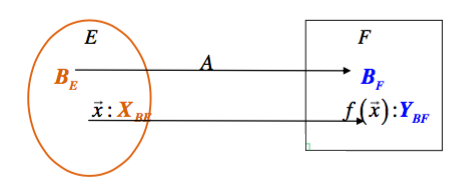
\includegraphics[height=3cm]{aplicacio_lineal}
\end{figure}
\[f(B_E) = B_F \cdot A\]

 \end{frame}    
 
 
 
  
    \begin{frame}
  \frametitle{Planteamiento general}
Se puede demostrar que 
\[A\cdot X_{BE} = Y_{BF}\]
 \end{frame}    

\subsection{Definici\'on}
  
    \begin{frame}
  \frametitle{Ecuaci\'on matricial de una aplicaci\'on lineal}
\begin{block}{Ecuaci\'on matricial}
\[A\cdot X_{BE} = Y_{BF}\]
Es la \textbf{ecuaci\'on matricial} de la aplicaci\'on lineal que relaciona las coordenadas de un vector $\vec x\in E$ en una base $B_E$ con las coordenadas $f(\vec x)$ en una base $B_F$.
\end{block}
 \end{frame}    
   
    \begin{frame}
  \frametitle{Ecuaci\'on matricial de una aplicaci\'on lineal}
\begin{block}{Teorema}
Sea $A\in M_n(\mathbb K)$ una matriz cuadrada de tama\~no $n$. Son equivalentes
\begin{itemize}
\item $A$ es invertible
\item Los vectores columna de la matriz $A$ son una base de $\mathbb K^n$ 
\item La aplicaci\'on lineal definida por: 
\[
  \begin{array}{@{}r@{\;}c@{\;}c@{\;}l@{}}
    f_A: & \mathbb K^n & \rightarrow & \mathbb K^n,   \\
       & X & \mapsto     & AX.
  \end{array}
\] 
Es biyectiva. 
\end{itemize}
\end{block}
 \end{frame}    
 
     \begin{frame}
  \frametitle{Ecuaci\'on matricial de una aplicaci\'on lineal}
\begin{block}{Teorema}
Sea la aplicaci\'on lineal  $f:E\longrightarrow F$, 
\begin{itemize}
\item $A$ la matriz de la aplicaci\'on lineal en las bases $B_E$ y $B_F$, 
\item $C$ la matriz de la aplicaci\'on lineal en otras bases $B_E'$ y $B_F'$, 
\item $P$ la matriz de cambio de base de $B_E'$ a $B_E$ ($B_E'\xrightarrow{P}B_E$),
\item $Q$ la matriz de cambio de base de $B_F'$ a $B_F$ ($B_F'\xrightarrow{Q}B_F$).
\end{itemize}
Entonces $Q^{-1}\cdot A \cdot P = C$

\end{block}
 \end{frame}    
 
  
\begin{frame}
\frametitle{Ecuaci\'on matricial de una aplicaci\'on lineal}
\begin{figure}[h]
\label{fig:volumen}
\caption{$Q^{-1}\cdot A \cdot P = C$}
\centering
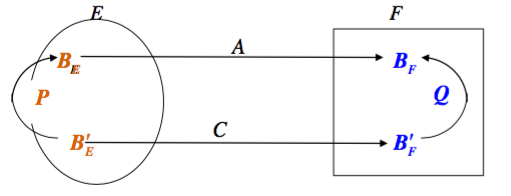
\includegraphics[height=3cm]{canvi}
\end{figure}
 \end{frame}   
 
 
      \begin{frame}
  \frametitle{Ecuaci\'on matricial de una aplicaci\'on lineal}
\begin{block}{Demostraci\'on}
\begin{itemize}
\item Ecuaci\'on matricial de la aplicaci\'on lineal para $A$, $B_E$ y $B_F$: $A \cdot X_{BE} = Y_{BF}$.
\item Ecuaci\'on matricial de la aplicaci\'on lineal para $C$, $B_E'$ y $B_F'$: $C \cdot X_{BE}' = Y_{BF}'$.
\item Ecuaci\'on de cambio de base de $B_E'$ a $B_E$ ($B_E'\xrightarrow{P}B_E$), $X_{BE} = P \cdot X_{BE}'$
\item Ecuaci\'on de cambio de base de $B_F'$ a $B_F$ ($B_F'\xrightarrow{Q}B_F$), $Y_{BF} = Q \cdot X_{BF}'$
\end{itemize}
\end{block}
 \end{frame}    
 
       \begin{frame}
  \frametitle{Ecuaci\'on matricial de una aplicaci\'on lineal}
\begin{block}{Demostraci\'on}
\[A \cdot X_{BE} = Y_{BF}\]
\[X_{BE} = P \cdot X_{BE}'\]
Por tanto: 
\[A \cdot ( P \cdot X_{BE}') = Y_{BF}\]
Adem\'as: 
\[Y_{BF} = Q \cdot Y_{BF}'\]
Por ello:
\[A \cdot (P\cdot X_{BE}') = Q\cdot Y_{BF}'\]
\end{block}
 \end{frame}    


        \begin{frame}
  \frametitle{Ecuaci\'on matricial de una aplicaci\'on lineal}
\begin{block}{Demostraci\'on}
Multiplicando los dos lados por $Q^{-1}$ y aplicando la propiedad asociativa del producto de matrices se obtiene: 
\[ (Q^{1} \cdot A \cdot P )\cdot X_{BE}' =  Y_{BF}'\]
Que es la ecuaci\'on matricial de $f$ en $B_E'$ y $B_F'$. Por tanto $Q^{1} \cdot A \cdot P $ ser\'a la matriz asociada a $f$ en estas bases:
\[Q^{1} \cdot A \cdot P =C\]
\end{block}
 \end{frame}    
 
         \begin{frame}
  \frametitle{Ecuaci\'on matricial de una aplicaci\'on lineal}
\begin{block}{Corolario}
Sea la aplicaci\'on lineal $f:E\longrightarrow E$ y sean:
\begin{itemize}
\item $A$ la matriz de la aplicaci\'on lineal en la base $B_E$, 
\item $C$ la matriz de la aplicaci\'on lineal en la base $B_E'$, 
\item $P$ la matriz de cambio de base de $B_E'$ a $B_E$ ($B_E'\xrightarrow{P}B_E$),
\end{itemize}
Entonces se cumple que: 
\[P^{-1}\cdot A \cdot P = C\]
\end{block}
 \end{frame}    
 
 \begin{frame}
\frametitle{Ecuaci\'on matricial de una aplicaci\'on lineal}
\begin{figure}[h]
\label{fig:matriz de cambio}
\caption{$P^{-1}\cdot A \cdot P = C$}
\centering
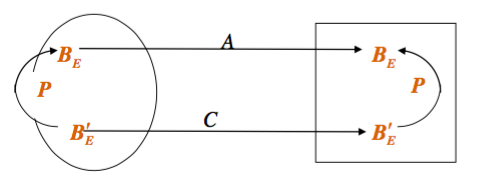
\includegraphics[height=3cm]{canvi_2}
\end{figure}
 \end{frame}   
 
 
          \begin{frame}
  \frametitle{Ecuaci\'on matricial de una aplicaci\'on lineal}
\begin{block}{Ejercicios}
Sea la aplicaci\'on lineal $f:\mathbb R^2 \longrightarrow \mathbb R^3$ dada por $f(x,y)= (x+y, y-2x, x+y)$. Encu\'entrese la matriz de $f$ respecto de la base can\'onica de $\mathbb R^2$ y la base $B_F = \{(1,1,0),(0,1,1),(0,0,-2)\}$ de $\mathbb R^3$.
\end{block}
 \end{frame}    
 
 
           \begin{frame}
  \frametitle{Ecuaci\'on matricial de una aplicaci\'on lineal}
Sea $A$ la matriz de $f$ asociada en las bases can\'onicas (calculada en un ejercicio anterior)
\[ A= \left(\begin{array}{rr}1 & 1 \\-2 & 1 \\1 & 1\end{array}\right)\]
$P$ es en este caso la matriz identidad de orden 2 (de la base can\'onica a ella misma) y $Q$ la matriz de cambio de base de $B_F$ a la base can\'onica de $\mathbb R^3$ ($B_F\xrightarrow{Q} B_C$)

\[ Q= \left(\begin{array}{rrr}1 & 0& 0 \\1 & 1 & 0 \\0 & 1 & -2\end{array}\right)\]
 \end{frame}    


           \begin{frame}
  \frametitle{Ecuaci\'on matricial de una aplicaci\'on lineal}

\begin{figure}[h]
\label{fig:last_ex}
\centering
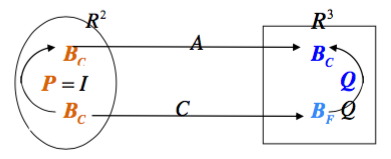
\includegraphics[height=3cm]{canvi_3}
\end{figure}

 \end{frame}    
 
 
 
 
\begin{frame}
\frametitle{Ecuaci\'on matricial de una aplicaci\'on lineal}
Entonces:
\[ C = Q^{-1} A P = \left(\begin{array}{rrr}1 & 0& 0 \\-1 & 1 & 0 \\-1/2 & 1/2 & -1/2\end{array}\right) \left(\begin{array}{rr}1 & 1 \\-2 & 1 \\1 & 1\end{array}\right)  \left(\begin{array}{rr}1 & 0 \\0 & 1 \end{array}\right) = \]
\[ \left(\begin{array}{rr}1 & 1 \\-3 & 0 \\-2 & -1/2\end{array}\right)  \left(\begin{array}{rr}1 & 0 \\0 & 1 \end{array}\right) = \]
\[ \left(\begin{array}{rr}1 & 1 \\-3 & 0 \\-2 & -1/2\end{array}\right)\]

 \end{frame}    
 
 
 
%  \begin{figure}[h]
  %  \label{fig:volum}
%\centering
%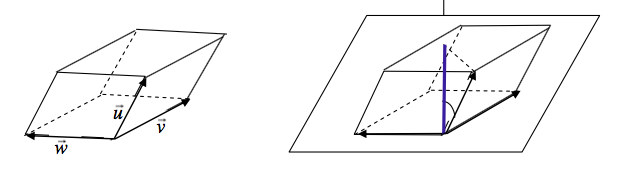
\includegraphics[height=3cm]{volum}
%\end{figure}


\end{document}